%!TEX root = ../phd-thesis-lei-ma.tex
%!TeX spellcheck = en-US
\chapter{Introduction}
\label{introduction}

\section{The Little Neutral One}

The neutrino has been one of the most interesting particles that has ever been discovered. Its fanscinating history started with the observation of beta decay, i.e., the emission of electrons in nuclear decays, such as
\begin{equation*}
% {}^A_Z \mathrm X \to {}_{Z+1}^A\mathrm X + e^- +\bar \nu_e .
{}^{14}_{6} \mathrm C \to {}^{17}_{7}\mathrm N + \mathrm e^{-} + \bar\nu_{\mathrm e}.
\end{equation*}
The fact that the electron energy spectrum in the beta decay process is continuous indicates the existence of a third product other than ${}^{17}_{7}\mathrm N$ and $\mathrm e^-$. In 1930, Pauli wrote a letter to a workshop in Tubingen explaining to the ``Radioactive Ladies and Gentlemen" about his so called ``neutron" as the missing particle in beta decay at that time. It was then called the neutrino since the name ``neutron" was latter used to name one of the nucleons. The missing particle $\bar\nu_{\mathrm e}$ in beta decays was then proven to be the anti-neutrino. In nuclear beta decays, the charged current weak interaction converts a down quark in the neutron to an up quark while releasing an electron and an anti-electron neutrino,
\begin{equation}
n\to p + e^- + \bar \nu_e .
\end{equation}
More generally, the positron/electron emission and capture processes are all neutrino-related nuclear reactions which are listed in Table~\ref{table:Neutrino_Reactions}. There are three different flavors of neutrinos, namely the electron flavor, the muon flavor, and the tau flavor as shown in Table~\ref{table:neutrino-properties}. The first direct detection of neutrinos was done by Clyde Cowan and Frederick Reines in 1956~\cite{Cowan1956} who used nuclear reactor neutrinos as the source of the experiment.

\begin{table}[ht]
\centering
 \begin{tabular}{ c  c  c}
 \hline
 \hline
 Reaction Type & Process & Mediator(s)   \\
 %[0.5ex]
 \hline
 Electron emission & ${}^A_Z X \to {}^A_{Z+1}X' + e^- +\bar \nu_e$ & $W^{\pm}$  \\
 Positron emission & ${}^A_Z X \to {}^A_{Z-1}X' + e^+ + \nu_e$ & $W^{\pm}$  \\
 Electron capture & ${}^A_Z X + e^- \to {}^A_{Z-1}X'  + \nu_e$ &  $W^{\pm}$ \\
 Positron capture & ${}^A_Z X + e^+ \to {}^A_{Z+1}X'  + \bar\nu_e$ &  $W^{\pm}$ \\
 [0.5ex]
 \hline

 $e^{\pm}$ annihilation &  $e^- + e^+  \to \nu + \bar\nu $  & $W^{\pm}$, $Z$ \\
%  Electron annihilation &  $e^- + e^+  \to \nu + \bar\nu $  & $Z$ \\
 Bremsstrahlung & $X+X' \to X + X' + \nu + \bar\nu$ & $Z$ \\
 [0.5ex]
 \hline

  $\nu (\bar\nu)$ capture & ${}^A_{Z}X + \overset{(-)}{\nu_e} \to {}^A_{Z\mp 1}X' + e^\pm $ & $W^{\pm}$\\
  [1ex]
 \hline
 $e^\pm\nu$ scattering & $e^- + \overset{(-)}{\nu} \to e^- + \overset{(-)}{\nu} $ &  $W^{\pm}$, $Z$ \\
 % $e^\pm\nu$ scattering & $e^{\pm} + \overset{(-)}{\nu_e} \to e^{\pm} + \overset{(-)}{\nu_e} $ &  $Z$ \\
 Nucleon scattering & $ {}^A_Z X + \overset{(-)}{\nu} \to {}^A_Z X + \overset{(-)}{\nu} $ &  Z\\
 [0.5ex]
 \hline
 \hline
 \end{tabular}
 \caption{Neutrino related nuclear and leptonic reactions.}
\label{table:Neutrino_Reactions}
\end{table}

\begin{table}[ht]
\centering
 \begin{tabular}{ c  c  c}
%  \hline
%  Property & Equation & Boson   \\ [0.5ex]
 \hline
 \hline
 [0.5ex]
  Electric Charge & 0\\
 [0.5ex]
  % \hline
  Spin & $1/2$ \\
 [0.5ex]
% \hline
 Mass & $<2~\mathrm{eV}$ \\
 [0.5ex]
 % \hline
 Interactions & Weak, Gravitation  \\
 % \hline
 [0.5ex]
 Flavors & $\nu_e$, $\nu_\mu$, $\nu_\tau$ \\
 % \hline
 [0.5ex]
 Chirality & Left \\
 [0.5ex]
 % \hline
 Hypercharge & $-1$ \\
 [0.5ex]
 \hline
 \hline
 \end{tabular}
 \caption{The physical properties of the neutrino~\cite{Patrignani:2016xqp}.}
\label{table:neutrino-properties}
\end{table}

\section{Stellar Neutrinos}


Besides man-made sources, neutrinos are also produced in many astrophysical environments.% Astrophysical neutrino sources such as stars, AGN, Gamma-ray bursts, and supernovae reveal a great amount of information about these sources. Though neutrinos interact very weakly with matter and are hard to detect, it is important to theoretically inspect neutrino productions in astrophysical processes.
For example, numerous nuclear reactions occur in stellar cores which produce luminous neutrino fluxes. %In this section, the nuclear reactions in stars are reviewed as the background of neutrino oscillations in matter.
% \subsection{Nuclear Reactions in Sun and Solar Neutrino Flux}
The most important nuclear reactions in the Sun are the pp chain reactions which are shown in Fig.~\ref{fig:pp_Chain_Branching}. In order to calculate the neutrino spectrum we need the neutrino production rate in each reaction and the branching ratios. Solar neutrinos are mostly produced in the pp reaction, Be electron capture and B decay which are labeled in red in Fig~\ref{fig:pp_Chain_Branching}:
\begin{align*}
&\mathrm{p+p\to {}^2H + e^+ +\nu_e}  & \mathrm{\leq 0.422MeV},\\
&\mathrm{{}^7Be + e^- \to {}^7Li + \nu_e} &\text{0.862MeV for 90\%},\\
&&\qquad \text{0.384MeV for 10\%}, \\
&\mathrm{{}^8B \to {}^8Be^* +e^+ +\nu_e}  & \mathrm{\leq 15 MeV}.
\end{align*}




\begin {figure*}%[!hbtp]
\centering
\begin{adjustbox}{width=\textwidth}
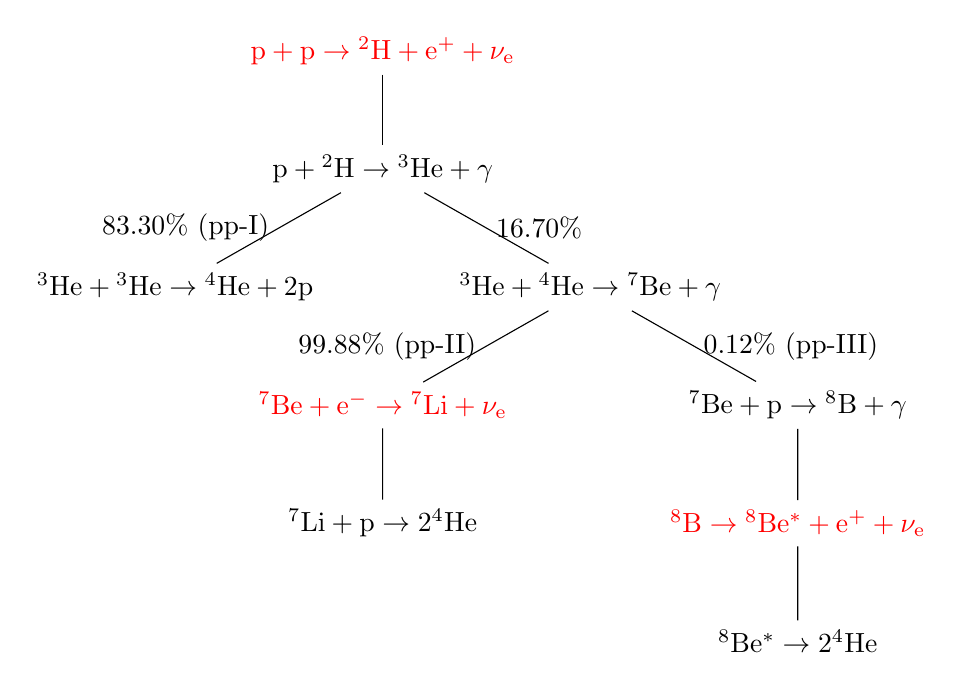
\begin{tikzpicture}[sibling distance=15em,
  every node/.style = {shape=rectangle,
    draw, align=center}
  edge from parent/.style = {draw, -latex},]]
  \node {\color{red}$\mathrm{p+p\to {}^2H + e^+ +\nu_e}$ }
    child { node {$\mathrm{p+{}^2H \to {}^3He + \gamma}$}
      child { node {$\mathrm{{}^3He+{}^3He \to {}^4 He + 2p }$}
          edge from parent node [left] {83.30\% (pp-I) } }
      child { node {$\mathrm{{}^3He+{}^4He \to {}^7 Be + \gamma }$}
        child { node {
\color{red}$\mathrm{{}^7Be + e^- \to {}^7Li + \nu_e}$
        }
        child { node { $\mathrm{{}^7Li + p \to 2{}^4He }$} }
        edge from parent node [left] {99.88\% (pp-II) } }
        child { node { $\mathrm{{}^7 Be + p \to {}^8 B + \gamma}$}
        child { node { \color{red}$\mathrm{{}^8B \to {}^8Be^* +e^+ +\nu_e}$ }
		child { node { $\mathrm{{}^8Be^* \to 2 {}^4He }$ } }}
        edge from parent node [right] {0.12\% (pp-III) } }
        edge from parent node [right] {16.70\%  } }};
\end{tikzpicture}
\end{adjustbox}
\caption{The pp chain reactions with the corresponding branching ratios. The branching ratios are taken from Ref.~\cite{Altmann2001}. }
\label{fig:pp_Chain_Branching}
\end{figure*}


% \begin{figure}[!hbtp]
% \centering
% 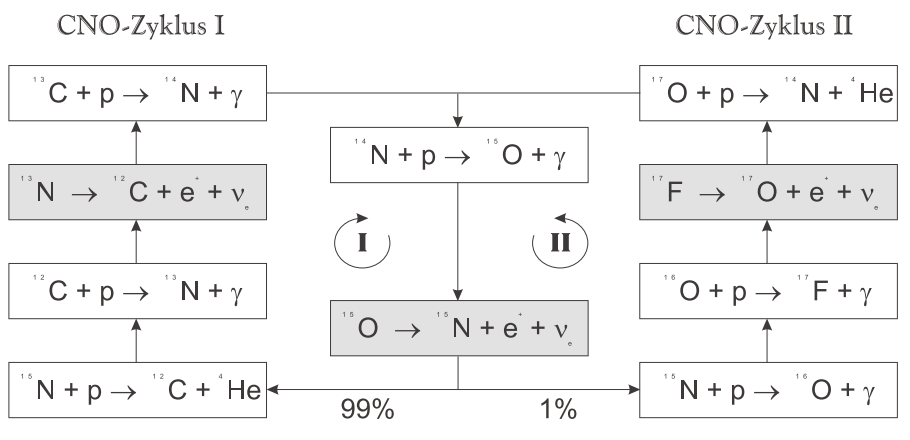
\includegraphics[width=\columnwidth]{chapters/assets/solar/cno_cycle.png}
% \caption{CNO cycle illustration~\cite{Adelberger2011a}.}
% \label{fig:cno_cycle}
% \end{figure}


Even without the knowledge of the detailed reactions, the conservation of the electric charge and the electron lepton number will lead to the overall neutrino production formula
\begin{equation}
\mathrm{4p+2e^- \to {}^4He + 2\nu_e }.
\end{equation}
It is important to notice that two neutrinos are emitted for each $\alpha$ particle, i.e., ${}^4\mathrm{He}$, produced in the Sun. Using this simple relation, we can estimate the neutrino number flux emitted by the Sun. The energy released during the production of each $\alpha$ particle is the difference between the initial and final rest masses of the particles,
\begin{equation}
Q=4m_p+2m_e-m_{\alpha}=26.7\mathrm{MeV},
\end{equation}
where the mass of the neutrinos are neglected. On average, each neutrino carries away an energy of $0.2\mathrm{MeV}$ and the rest of the energy is in the form of thermal energy $Q_\gamma=26.3\mathrm{MeV}$~\cite{Adelberger2011a}. %Energy flux density of solar photons near Earth is given by the solar constant $S_0$.
Since two neutrinos are emitted for the production of thermal energy $Q_\gamma$, the number flux of the solar neutrinos near the Earth is approximately
\begin{equation}
\Phi_\nu = \frac{2 S_0}{Q_\gamma} \approx 6\times 10^{10} \mathrm{cm^{-2}s^{-1}},
\end{equation}
where the solar constant $S_0$ is the energy flux of solar photons on the top of the Eath atmosphere.
%Neutrinos are hard to detect but a large number flux makes it possible to detect solar neutrinos~\cite{Cleveland1998,Lande2003,McDonald2013}.

% On the other hand, the solar neutrinos have a certain energy spectrum due to the composition of nuclear reactions. Inside our Sun, two additional reactions other than pp neutrinos also produce neutrinos which are called pep and hep neutrinos.
% \begin{itemize}
% \item pep neutrinos are produced in
% \begin{equation}
% \mathrm{p + e^- + p \to {}^2H +\nu_e},
% \end{equation}
% which only has a branching ratio 0.4\% instead of the 99.6\% of pp reaction.
% \item hep neutrinos are produced in
% \begin{equation}
% \mathrm{ {}^3He + p \to {}^4He + e^+ \nu_e },
% \end{equation}
% which has a branching ratio of $2\times 10^{-5}\%$. As a comparison, the $\mathrm{{}^3He + {}^3He}$ has a branching ratio $85\%$ and $\mathrm{{}^3He + {}^4He}$ has a branching ratio $15\%$.
% \end{itemize}


As the detection of neutrinos became feasible, Ray Davis and John Bahcall et al worked out the solar neutrino flux and led the Homestake experiment to measure the solar neutrinos. The results revealed that the neutrino flux detected was less than what was predicted by the standard solar model~\cite{Bahcall1973}. This is the solar neutrino problem. It is now known that the solution to the problem is related to the neutrino. The electron neutrinos produced in the solar core transform to other flavors while they travel to the Earth. This phonomenon is referred known as the flavor transformation of the neutrino, or neutrino oscillations. The theory of neutrino oscillations was first proposed by Pontecorvo in 1968~\cite{Pontecorvo1968}. The field of neutrino oscillations has grown significantly into a broad field in physics since then.



\section{Supernova Neutrinos}


Another astronomical source of neutrinos is the core-collapse supernova explosion. Massive stars with masses larger than 6−8 solar masses are very bright. However, violent delights have violent ends. When the core of a massive star runs out of nuclear fuel, it collapses under its own gravity. During the collapse, the inner core is compressed to almost nuclear density, which has a stiff equation of state. The materials falling onto the highly compressed inner core are bounced outward which generates a shock wave and may lead to an explosion. However, supernova simulations to date show that the shock wave itself is not always energetic enough to produce the explosion~\cite{Janka2016b}. In most cases, it stalls and becomes a standing accretion shock wave. To revive the shock, more energy has to be deposited behind the shock. A possible solution is to introduce reheating of the shock by neutrinos~\cite{Janka2016b}. In fact 99\% percent the energy released in a core-collapse supernova is carried away by neutrinos.
%Those explosions are the most luminous sources of neutrinos in the universe~\cite{Raffelt1996wa}.
In order to implement the neutrino-driven mechanism in computer simulations of supernovae, the flux and flavor content of the neutrinos have to be known everywhere behind the shock. Thus neutrino oscillations in dense matter become a key to the supernova explosion problem.

The average energy of the neutrinos $\langle E \rangle$ emitted during a supernova explosion is of the order of 10MeV~\cite{Janka2017}, and the neutrino luminosity at the early epoch is approximately $10^{52}\mathrm{ergs\cdot s^{-1}}$~\cite{Pejcha2012a}.
% The supernova explosion releases neutrinos with energy flux on the order of $10^{51}\mathrm{ergs\cdot s^{-1}}$~\cite{Bethe1985}.
Therefore, the number density of the neutrinos at the radius $R$ is
\begin{equation*}
   n \sim  10^{18} \mathrm{cm^{-3}} \left(\frac{100\mathrm{km}}{R}\right)^2 \left(\frac{10\mathrm{MeV}}{\langle E \rangle}\right).
\end{equation*}
% which corresponds to the number flux
% \begin{equation*}
%   \Phi \sim 10^{27} \mathrm{cm^{-2} s^{-1}}\left(\frac{100\mathrm{km}}{R}\right)^2 \left(\frac{10\mathrm{MeV}}{\langle E \rangle}\right).
% \end{equation*}
% Compared to the neutrino flux at the surface of the Sun, which is of the order $10^{15}\mathrm{cm^{-2} s^{-1}}$, supernova neutrinos is much denser.
It turns out that the ambient dense neutrino medium has a significant impact on neutrino oscillations, which has been intensely investigated in the last decade~\cite{Duan2010}.

Observation-wise, the neutrino signals from a galactic supernova can reveal a great amount of information about the physical conditions inside the supernova. In fact, the detection of supernova neutrinos is on the task list of the Deep Underground Neutrino Experiment (DUNE)~\cite{Kemp2017}.




\section{Organization of the Disseration}


% As we have seen, it is crucial to understand neutrino flavors.
The rest of the disseration is organized as follows.
In Chapter~\ref{chap:basics}, I will review neutrino oscillations in vacuum and in environments with smooth matter density profiles.
% Meanwhile, neutrino oscillations are ingredients of many other astrophysical, cosmological, and astronomical problems, such as neutron star mergers, dark matter, nucleosynthesis, etc. In order to gain a better understanding of neutrinos in these exotic environments, neutrino oscillations in dense matter background and dense neutrino background have to be thoroughly investigated. The seminal work by Mikheev--Smirnov--Wolfenstein proved neutrino interactions with matter background have significant effect on neutrino oscillations. They showed that neutrinos propagating through decreasing matter density experience a potential that alters the flavor conversions (MSW effect), which may also lead to maximum conversions between flavors~\cite{Mikheev:1986gs,wolf78,wolfensteinprd1979}. It is also know that neutrino oscillations in more general matter density profiles exhibit interesting phenomena. Resonances are found as the characteristic length scale in matter density profile and characteristic length scale of the neutrinos satisfies certain relations.
In Chapter~\ref{chap:matter}, I will discuss my work on neutrino oscillations in oscillatory matter profiles, which can be decomposed into Fourier modes and interpreted as a superposition of Rabi oscillations.
%Apart from dense matter background, neutrinos also interact with neutrinos themselves and introducing nonlinear dynamics. The neutrino self-interactions are analyzed using linear stability analysis.
In Chapter~\ref{chap:collective}, I will first review how neutrino self-interactions can cause a dense neutrino medium to oscillate collectively. Then I will discuss my study on the dispersion relations of the collective modes of neutrino oscillations.
%, as well as the dispersion relations in linear stability analysis. I will also discuss the neutrino halo problem. The halo problem exists because neutrino propagating out of dense matter medium will be scattered and forming a neutrino halo. Some of the neutrinos will propagate backward and interact with forward propagating neutrinos and alter the neutrino flavors. Mathematically speaking, the neutrino halo problem is a nonlocal boundary value problem. I will explain the numerical relaxation scheme that we developed, which we have proven to be a promising method to solve neutrino halo problem.
I will also discuss a premilinary work on neutrino oscillations when both forward and backward neutrino fluxes are present.
In Chapter~\ref{chap:conclusion}, I will summarize my work and discuss possible future directions of the field.
